\documentclass[a4paper,10pt, twocolumn]{article}
\usepackage{amsmath}
\usepackage{graphicx}
\usepackage[font={small,it}]{caption}
\usepackage{titling}

\begin{document}
\setlength{\droptitle}{-100pt}
\author{Alun Meredith\vspace{-2ex}% Toggle commenting out the command
}
\date{March 17, 2016 \vspace{-4ex}}
\title{Coursework 1: Analysis of visualisations\vspace{-2ex}% to see the effect
}
\maketitle
\small

\section{Introduction}
The corpus analysed is a collection of 24 books about antiquity, written in the 18-19th Century. Many are translations of older texts and often volumes of a larger book. The data is html documents of OCR scans from the Google Books Library Project, separated into each page.

Manually extracting some metadata about each book (title, author, translator, year written, year translated) we can see some themes worth investigating: If it is written about/by a Roman or not, written in/about antiquity, volumes within a series, written by the same author, effect of different translators.
\section{Preprocessing}
To extract the text from each html page, xml2 was used. Using html tags to isolate the second paragraph (class = 'ocr\_par'), which contained the body of text without the title. The 'ocr\_cinfo' contained each word separately to avoid an error where words across newlines were merged with a naive approach. Pages were concatenated to produce books.

Using the 'tm' package a raw corpus was built from these vectors. After casefolding, whitespace, non-alphabetic characters and stopwords were removed. Stopwords removed were tm's "english", numbers and common artefacts of the OCR. A regular expression was used to remove Roman numerals and words were stemmed.

Producing a term-document matrix for 1-3 ngrams, removing sparse terms and using TF-IDF\footnote{Different sparsity levels used for different purposes, analysis run both with and without TF-IDF} before producing a cosine dissimilarity matrix. 

\begin{figure}
	\includegraphics[width=0.7\linewidth]{entropy.png}
	\centering
	\caption{Shannon Entropy of each document, coloured by book each volume belongs to. Full names on github}
	\label{fig:entropy}
\end{figure}  

\subsection{Entropy}
The Shannon entropy \textbf{CITE} was computed on each book before the stopwords had been removed using the entropy package. 

We can see that within the 5 terms with the highest entropy are the dictionary/encyclopedia style books which are expected to have the highest information density. In addition volumes of the same book are generally ranked close together with the exception of Josephus IV and Tacitus History IV, the later of which is quite a remarkable outlier. Cases where the translator changes for volumes of the same book doesn't have a noticeable impact (E.g. Decline \& Fall 4 vs. 1,3,5). This suggests there isn't a strong component of things being translated in totally different ways. 

\subsection{Clustering}
Both hierarchical  and K-means clustering was completed using the packages "agnes" and "cluster". 

\begin{figure}
	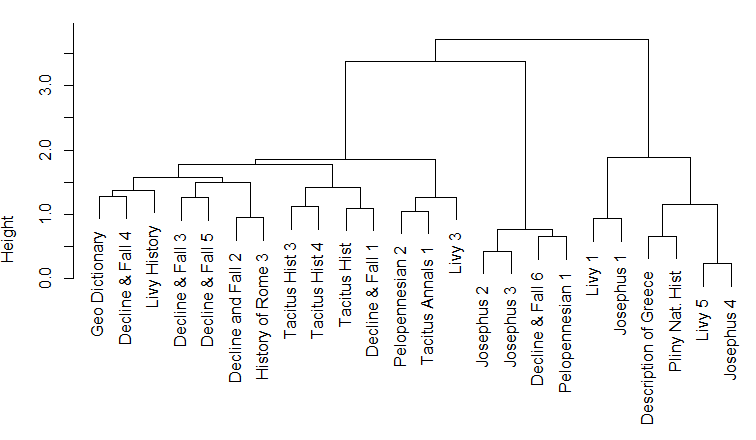
\includegraphics[width=0.9\linewidth]{dendorgram.png}
	\centering
	\caption{Dendrogram of agglomerative hierarchical  clustering using "Ward" method and cosine distance metric. Produced from hclust base function in R.}
	\label{fig:heir}
\end{figure} 

The hierarchical  clustering (fig. \ref{fig:heir}) used the "Ward" method although other methods were used with the same clusters (except single linkage). There are 3 main clusters, looking at their highly weighted terms we can see that they can be described as Jewish: Jew, Herod, etc; Non-Roman:Arab, Constantinople, Peloponnesan; Roman: loosely clustered. These clusters can be unstable to small changes, upon identifying and merging two spellings of constantnopl Livy I and Josephus I joined the non-Roman cluster. Decline \& Fall I and Tacitus Hist III are linked through the trigram "see geographic table". 

Unlike the entropy measure which grouped volumes of a book together well, hierarchical clustering with TF-IDF is grouping on topic rather than language style. 

Before TF-IDF many highly weighted words are similar to stopwords such as "there". However there are useful defining words highly weighted as well such as "citi" and "town" under the geographic dictionary \footnote{A list of the 10 highest weighted words being referred to for different weighting schemes and ngrams on github.com/alunmeredith}. Therefore we can try to get access to some of the language instead of the topics by enforcing relatively low sparsity and not using TF-IDF. \textbf{move / complete plots / analysis} 

Using 3 clusters after computing an elbow plot (fig. \ref{fig:elbow}), this also matches the clusters from the hierarchical clustering. 



\begin{figure}
	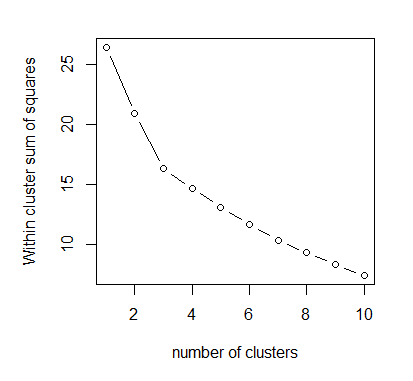
\includegraphics[width=0.7\linewidth]{elbow.png}
	\centering
	\caption{Elbow plot varying number of clusters vs. within cluster spread}
	\label{fig:elbow}
\end{figure}



\begin{figure}
	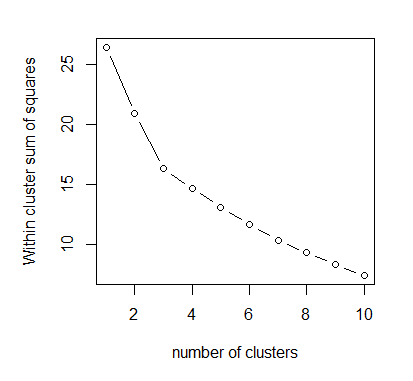
\includegraphics[width=0.7\linewidth]{elbow.png}
	\centering
	\caption{K-means clustering plotted on First two principal components. Using cluster package in R. }
	\label{fig:kmeans}
\end{figure} 
 
\section{Conclusion}
There are two main aspects in which this work can be clustered, on the language/style used within the document or on the topic. We have seen clustering and dimensionality reduction techniques, especially using TF-IDF can extract topical information whereas entropy better groups language style of volumes within a book. We also saw how TF-IDF clustering was sensitive to singular words (e.g. Constantinople). \textbf{it may therefore be wise to suppress some of the scaling of these weights with frequency}

As TF-IDF weights names so heavily (due to their sparsity in documents they are not important in) further work proposed (not able to complete) is to use these bigram terms to query dbpedia, if matching a person then extract a year of death/birth and plot the distribution of these for each book.

We have seen no clear patterns to distinguish works produced vs. translated or effects of different translators. However because language style was difficult to access. 
\bibliographystyle{abbrv}
\bibliography{sigproc}

\end{document}
